\documentclass[notes]{beamer}
\usepackage[latin1]{inputenc}
\usepackage{tikz}
\usetikzlibrary{arrows}
\usetikzlibrary{shapes.misc}
\usepackage{verbatim}
\usepackage{amsthm}
\usetheme{Warsaw}

\title{Homogeneity is Independent from Randomness}
\author{Li Ling Ko}
\institute{University of Notre Dame}
\date{22 January, 2018}
\setbeamertemplate{footline}[frame number]
\setbeamertemplate{theorems}[numbered]

\newcommand{\TODO}[1]{\textcolor{red}{TODO: #1}}
\newtheorem{thm}{Theorem}
\newtheorem*{thm*}{Theorem}
\newtheorem*{main-thm*}{Main Theorem}
\newtheorem{coro}{Corollary}
\newtheorem*{coro*}{Corollary}
\newtheorem{pf}{Proof}
\newtheorem*{pf*}{Proof}
\newtheorem{define}{Definition}
\newtheorem*{define*}{Definition}
\newtheorem{claim}{Claim}
\newtheorem*{claim*}{Claim}
\newtheorem{Fact}{Fact}
\newtheorem*{Fact*}{Fact}

\begin{document}
\begin{frame}
  \titlepage
\end{frame}

\begin{frame}{Notations}
  \begin{itemize}
    \item $\omega=\mathbb{N}$, $a,b,\ldots\in\omega$,
      $A,B,\ldots\subseteq\omega$, $\sigma,\tau\in\omega^{<\omega}$,
      $\mathcal{A},\mathcal{B},\ldots\subseteq\omega^\omega$.
    \item Trees $T$ are subsets of $\omega^{<\omega}$ closed under initial
      segments; i.e. $\sigma^{\frown}n\in T \rightarrow \sigma\in T$.
    \item Paths are functions $f:\omega\rightarrow\omega$. A tree contains
      a path $f$ iff $T$ contains every initial segment $f\restriction n
      \prec f$.
    \item $[T] :=\{f:f\; \text{is a path in}\; T\}$, $[\sigma]:=\{f:f\;
      \sigma\prec f\}$.
    \item Turing functionals on trees are partial-recursive functionals
      $\Gamma:2^{<\omega}\rightarrow\omega^{<\omega}$ where
      $\tau\in\Gamma^{\sigma^\frown n} \rightarrow
      \tau\in\Gamma^{\sigma}$. $\Gamma$ can be extended naturally to
      $\Gamma:2^\omega\rightarrow\omega^{\omega}$.
    \item Given set $A$ and cardinal $\kappa$, $[A]^\kappa
      :=\{B\subseteq A: |B|=\kappa\}$.
    \item Given $A\in[\omega]^\omega$, we sometimes refer to $A$ by its
      characteristic function $c_A:\omega\rightarrow\{0,1\}$, or by its
      principal function $p_A:\omega\rightarrow\omega$, which is the
      strictly increasing function listing the elements of $A$.
  \end{itemize}
\end{frame}

\begin{frame}{Ramsey's Theorem ($\text{RT}$)}
  \begin{define*}[$c$-homogeneous]
    Given $k$-coloring $c:[\omega]^n\rightarrow k$, a subset
    $A\subseteq\omega$ is $c$-homogeneous if every $n$-tuple over $A$ is
    given the same color by $c$.
  \end{define*}

  \vspace{1em}
  \begin{thm*}[Ramsey's Theorem]
    Fix $n,k\leq1$. $\text{RT}_k^n$ is the statement that every $k$-coloring
    $c:[\omega]^n\rightarrow k$ has an infinite $c$-homogeneous set.\\
    RT is the statement $(\forall n)(\forall k)\; \text{RT}_k^n$.
  \end{thm*}

  \vspace{1em}
  RT asserts homogeneity exists.
\end{frame}

\begin{frame}{Randomness}
  Intuitively, a path $f\in2^\omega$ is random if it cannot be ``caught''
  by any descending enumeration of trees $2^{<\omega}\supseteq T_0\supseteq
  T_1\supseteq \ldots$, because such trees would reveal information on the
  sequences caught by all of them. A descending sequence is eligible to judge
  for randomness only if the trees shrink fast enough for the class of paths
  caught by all of them to be ``sparse'', because if too many paths are
  caught, the information on the paths is not useful.

  \vspace{1em}
  One way of formalizing the notion of a sparseness of a tree is:
  \begin{define*}
    A (measurable) binary tree $T\subseteq2^{<\omega}$ has positive measure
    if
    \[\lim_s \frac{|\{\sigma\in T: |\sigma|=s\}|}{2^s} >0.\]
  \end{define*}
\end{frame}

\begin{frame}{WWKL asserts Randomness}
  A series of trees $T_0\supseteq T_1\supseteq\ldots$ is eligible to
  test for randomness if the limit of their measures is 0. Since there are
  only countably many Turing machines that can give randomness tests,
  and the class of non-randoms from each test has measure 0, and the
  measure of a countable union of (measurable) classes of measure 0 is
  still 0, the class of non-randoms has measure 0.

  \vspace{2em}
  Thus if a (measurable) tree has positive measure, it must contain a
  random. Weak Weak Konig's Lemma (WWKL) asserts that at least one of its
  paths is random by stating
  \begin{thm*}[Weak Weak Konig's Lemma]
    Every binary tree with positive measure contains a path.
  \end{thm*}
\end{frame}

\begin{frame}{WWKL, WKL, KL}
  The paths of an instance of Weak Konig's Lemma (WKL), however, may
  all be non-randoms, because WKL includes also binary trees with measure
  0:
  \begin{thm*}[Weak Konig's Lemma]
    Every binary tree with infinite nodes contains a path.
  \end{thm*}

  \vspace{2em}
  Konig's Lemma includes even trees that are not binary:
  \begin{thm*}[Konig's Lemma]
    Every finitely-branching tree with infinite nodes contains a path.
  \end{thm*}
\end{frame}

\begin{frame}{Homogeneity versus Randomness}
  A natural question to ask is which of the statements RT, KL, WKL, WWKL is
  stronger. Intuitively, WKL is stronger than WWKL, because a binary tree
  of positive measure has infinite nodes, so if all binary trees with
  infinite nodes have a path, then those with positive measure must
  have one too. A question that is harder to answer is:
  \newtheorem*{question*}{Question}
  \begin{question*}
    Which notion is stronger, homogeneity or randomness?
  \end{question*}
  If a given a path is homogeneous, does that say anything about how random
  it is? Likewise, if a given path is random, will it necessarily provide
  information on finding homogeneous paths?

  \vspace{0.5em}
  Since the notions of homogeneity and randomness are captured by RT and
  WWKL respectively, we are essentially asking which of RT and WWKL is
  stronger.
\end{frame}

\begin{frame}{Problem, Instance, Solution}
  We formalize the notion of problems and the strength between them.

  \vspace{1em}
  \begin{define*}[Problem, instance, solution]
    A mathematical \textbf{problem} is a collection of \textbf{instances},
    with a collection of \textbf{solutions} for each instance.
  \end{define*}

  \vspace{1em}
  For example, RT is a problem; its instances are the collections of
  colorings $c:[\omega]^n\rightarrow k$ for every $n,k\in\omega$, and the
  solutions of each $c$ are the class of $c$-homogeneous paths.

  \vspace{1em}
  Similarly, WWKL is a problem; its instances are the collections of binary
  trees with positive measure, and the solutions of each instance is the
  class of paths in the tree.
\end{frame}

\begin{frame}{Strongly Omnisciently Computably Reducible
($\leq_{\text{soc}}$)}
  \begin{define*}[Strongly Omnisciently Computably Reducible]
    Problem \textbf{P} is \textit{soc}-reducible to problem \textbf{Q}
    (written \textbf{P} $\leq_{\text{soc}}$ \textbf{Q}) if for every
    \textbf{P}-instance \textit{I}, there is a \textbf{Q}-instance
    \textit{J} such that every solution to \textit{J} computes a solution
    to \textit{I}.
  \end{define*}

  $\leq_{\text{soc}}$ successfully captures this expected relation:
  \begin{center}
    WWKL $\leq_{\text{soc}}$ WKL $\leq_{\text{soc}}$ KL.
  \end{center}

  \vspace{0.5em}
  \textbf{WWKL $\leq_{\text{soc}}$ WKL:} Given a binary tree with
  positive measure, this tree has infinite branches and is therefore an
  instance of WKL. The desired relation follows from definition of
  $\leq_{\text{soc}}$.

  \vspace{0.5em}
  \textbf{WKL $\leq_{\text{soc}}$ KL:} Given a binary tree with infinite
  branches, this tree is finitely-branching and therefore an instance of
  WKL. The desired relation follows from definition of $\leq_{\text{soc}}$.
\end{frame}

\begin{frame}{KL, RT $\leq_{\text{soc}}$ WKL}
  WKL is powerful under $\leq_{\text{soc}}$. Given any KL or RT
  instance, fix one of its solutions, and choose the WKL instance whose only
  path codes that solution as an path in $2^\omega$. By definition of
  $\leq_{\text{soc}}$, the given instance reduces to this WKL instance.

  \vspace{1em}
  For example, given a KL instance, fix one of its solutions
  $f:\omega\rightarrow\omega$, code this solution as a path in $2^\omega$
  in a recoverable manner.

  \vspace{1em}
  For instance, if $f$ is $2,9,3,\ldots$, we can code $f$ as the path
  $110$ $1111111110$ $1110\ldots$.

  \vspace{1em}
  Similarly, any solution of an RT instance can be seen as an infinite
  subset of $\omega$. Its characteristic function will be a path in
  $2^\omega$.
\end{frame}

\begin{frame}{Homogeneity ``independent from'' Randomness}
  Dependencies under $\leq_{\text{soc}}$
  \vspace{2em}

  \begin{center}
    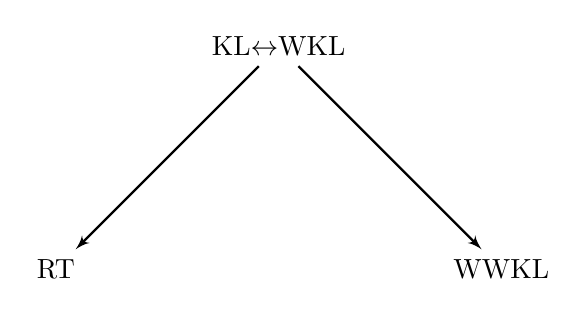
\begin{tikzpicture}[node distance=4cm,auto,thick,>=latex']
      \node (KL) {KL$\leftrightarrow$WKL};
      \node (WWKL) [below right of=KL] {WWKL};
      \node (RT) [below left of=KL] {RT};
      \draw[->] (KL) -- (RT);
      \draw[->] (KL) -- (WWKL);
      %\draw [->,red] (RT) -- coordinate (m) (WWKL);
      %\draw[shift={(m)},red](-0.1,-0.1)--(0.1,+0.1);
    \end{tikzpicture}
  \end{center}
\end{frame}

\begin{frame}{Bi-Hyperimmune sets}
  \begin{define}[Hyperimmune, Bi-hyperimmune]
    $A\subseteq\omega$ is \textit{hyperimmune} if its principal function
    $p_A$ cannot be dominated by any total recursive function. That is,
    there is no effective way of knowing when a new element of $A$ has
    appeared. $A$ is \textit{bi-hyperimmune} if both $A$ and $\bar{A}$ are
    hyperimmune.
  \end{define}

  \begin{thm}
    Bi-hyperimmune sets exist.
  \end{thm}

  \textbf{Pf:} Enumerate recursive functions $f_0,f_1,\ldots$. At stage
  $s$, let $i$ be the number of elements in $A$ and $\bar{A}$ that has been
  defined so far. Put enough elements into $\bar{A}$ till the $(i+1)$-th
  element of $A$ exceeds that of $f_s$, then put the next element into $A$.
  This ensures that $f_s$ cannot tell when the $(i+1)$-th element of $A$
  has appeared. Repeat with roles of $A$ and $\bar{A}$ reversed.
  $\blacksquare$
\end{frame}

\begin{frame}{Class of sets computing subsets of hyperimmune is null}
  \begin{thm}
    Given a hyperimmune set, the class of sets that can compute an
    infinite subsets null.
  \end{thm}

  \textbf{Proof idea:} Assume not. Then there are enough paths computing
  infinite subsets of $A$ such that we can effectively ask them to ``vote''
  for intervals that contain new elements of $A$. Thus effectively
  dominating $p_A$, $\Rightarrow\Leftarrow$.\\
  \vspace{1em}

  \textbf{Pf:} Fix Turing functional $\Phi$. Write $\mathcal{B} :=\{X:
  \Phi^X\in[A]^\omega\}$. Suffices to show $\mu(\mathcal{B})=0$. Assume
  $\mu(\mathcal{B})=4m>0$.
\end{frame}

\begin{frame}{Class of sets computing subsets of hyperimmune is null}
  \begin{itemize}
    \item Approximate $\mathcal{B}$ by open cover
      $\mathcal{O}\supseteq\mathcal{B}$ with
      $\mu(\mathcal{O}-\mathcal{B})<m$.
    \item Approximate $\mathcal{O}$ by basic open sets
      $[\sigma_0],\ldots,[\sigma_n] \subseteq\mathcal{O}$ with
      \[\mu(\mathcal{O}-([\sigma_0]\cup\ldots\cup[\sigma_n])) <m.\]
    \item Fix effective enumeration of branches $\sigma$ in
      $[\sigma_0]\cup\ldots\cup[\sigma_n]$.
    \item At stage $s=0$, wait till a measure of $2m$ of such $\sigma$'s
      finds an element via $\Phi$; let $f(0)$ be the largest element found.
    \item Since $[\sigma_0]\cup\ldots\cup[\sigma_n]$ approximate
      $\mathcal{B}$ tightly, such $\sigma$'s exist.
      \begin{align*}
        \mu(\text{``true'' voters})>2m,\\
        \mu(\text{``false'' voters})<2m.
      \end{align*}
      Thus $f(0)\geq p_A(0)$.
    \item At stage $s+1$, wait till a measure of $2m$ of $\sigma$'s
      finds an element $>f(s)$; let $f(s+1)$ be the largest
      element found. $\blacksquare$
  \end{itemize}
\end{frame}

\begin{frame}{RT $\nleq_{\text{soc}}$ WWKL}
  \begin{itemize}
    \item $\text{RT}_2^1$ $\nleq_{\text{soc}}$ WWKL
    \item Fix $A\in[\omega]^\omega$ where
      \begin{align*}
        &\mu(\{X: X\; \text{computes element in}\; [A]^\omega\}) =0,\\
        \text{and}\;\;\; &\mu(\{X: X\; \text{computes element in}\;
        [\bar{A}]^\omega\}) =0.\\
      \end{align*}
    \item Choose 2-coloring $c:\omega\rightarrow\{0,1\}$, $c(n)=0
      \Leftrightarrow n\in A$.
    \item Given any instance of WWKL, since the set of its paths has
      measure $>0$, some path must fail to compute any infinite
      homogeneous set of $c$. 
    $\blacksquare$
  \end{itemize}
\end{frame}

\begin{frame}{Recursive-Encodability, $\Pi_1^0$-Encodability}
  For the remaining directions
  \begin{itemize}
    \item WKL $\nleq_{\text{soc}}$ RT
    \item WWKL $\nleq_{\text{soc}}$ RT
  \end{itemize}
  we need the following definitions and characterizations:

  \begin{define}[Recursive-Encodable $A\subseteq\omega$]
    $A\subseteq\omega$ is recursively-encodable if given any
    $X\in[\omega]^\omega$, some subset of $X$ computes $A$.
  \end{define}

  \begin{define}[$\Pi_1^0$-encodable $\mathcal{A}\subseteq\omega^\omega$]
    $\mathcal{A}\subseteq \omega^{\omega}$ is $\Pi_1^0$-encodable if for
    every $X\in[\omega]^\omega$, there exists $Y\subseteq X$ and tree
    $T\leq_T Y$ such that
    \[\mathcal{A} \supseteq [T]\neq\emptyset,\]
    and some $f\leq_T Y$ bounds every branch in $T$.
  \end{define}
\end{frame}

\begin{frame}{Characterizing Encodability}
  \begin{main-thm*}[Characterizing $\Pi_1^0$-encodable
  $\mathcal{A}\subseteq\omega^\omega$]
    $\mathcal{A}\subseteq \omega^{\omega}$ compact. Then
    \[\mathcal{A}\; \text{is}\; \Pi_1^0\text{-encodable}\; \Leftrightarrow
    \mathcal{A}\; \text{contains}\; \Sigma_1^1\text{-subset}\;
    (\neq\emptyset).\]
  \end{main-thm*}

  \begin{coro*}[Characterizing Recursively-Encodable $A\subseteq\omega$]
    $A\subseteq\omega$ recursively-encodable $\Leftrightarrow$ $A$ is
    hyperarithmetic.
  \end{coro*}

  \vspace{1em}
  From Main Theorem, suffices to show
  \begin{itemize}
    \item $A\subseteq\omega$ is hyperarithmetic $\Leftrightarrow$
      $\{A\}\subseteq\omega^\omega$ is $\Sigma_1^1$
    \item $A\subseteq\omega$ recursively-encodable $\Leftrightarrow$
      $\{A\}\subseteq\omega^\omega$ is $\Pi_1^0$-encodable
  \end{itemize}
\end{frame}

\begin{frame}{$A$ hyperarithmetic $\Leftrightarrow$ $\{A\}$ is $\Sigma_1^1$}
  \begin{align*}
    \;&A\subseteq\omega\; \text{hyperarithmetic}\\
    \Rightarrow\; & A\in\Sigma_1^1\\
    \Rightarrow\; & A=\{n:(\exists f)(\forall s)\; [R(f\restriction s,n)]\}\\
    \Rightarrow\; & \{A\}= \{g:(\exists f)(\forall s)(\forall n)\\
    &[R(f\restriction s,n) \rightarrow g(n)=1 \wedge \neg R(f\restriction s,n)
      \rightarrow g(n)=0]\}\\
    \Rightarrow\; &\{A\}\subseteq\omega^\omega\; \text{is}\; \Sigma_1^1,\\
    &\\
    \Rightarrow\; & \{A\}= \{g:(\exists f)(\forall s)\; [Q(f\restriction
      s,g\restriction s)]\}\\
    \Rightarrow\; &
      \begin{cases}
        A=\{n:(\exists g)\; [g(n)=1\; \wedge\; (\exists f)(\forall s)\;
          Q(f\restriction s,g\restriction s)]\}\\
        A=\{n:(\forall g)\; [g(n)=0\; \rightarrow\; (\forall f)(\exists s)\;
          \neg Q(f\restriction s,g\restriction s)]\}\\
      \end{cases}\\
    \Rightarrow\; &A\in\Delta_1^1\\
    \Leftrightarrow\; &A\subseteq\omega\; \text{hyperarithmetic}.\;
    \blacksquare\\
  \end{align*}
\end{frame}

\begin{frame}{$A$ recursively-encodable $\Leftrightarrow$
$\{A\}$ is $\Pi_1^0$-encodable}
  \begin{align*}
    \;&A\subseteq\omega\; \text{recursively-encodable}\\
    \Leftrightarrow\; & (\forall X\in[\omega]^\omega)(\exists Y\subseteq
      X)\; [Y\geq_T A]\\
    \Rightarrow\; & (\forall X\in[\omega]^\omega)(\exists Y\subseteq X)\;
      [\{A\}=\{\Phi^Y\}]\\
    \Rightarrow\; &\{A\}\subseteq\omega^\omega\; \text{is}\;
      \Pi_1^0\text{-encodable},\\
    &\\
    \Rightarrow\; & (\forall X\in[\omega]^\omega)(\exists Y\subseteq
      X) [\{A\}=[R^Y]]
  \end{align*}
  Given $A\restriction n$, to decide if $n\in A$, enumerate all nodes
  $\sigma\in2^{<\omega}$ extending $A\restriction n$ and check if
  $R^Y(\sigma)$. Since $A$ is the unique path in $[R^Y]$, by weak Konig's
  lemma, eventually exactly one of $[(A\restriction n)^\frown 0]$ or
  $[(A\restriction n)^\frown 1]$ will be covered by a finite set of basic
  open covers $[\sigma_0]\cup\ldots\cup[\sigma_m]$ with $\neg R(\sigma_i)$.
  Then the other $[(A\restriction n)^\frown j]$ gives the correct value
  of $A(n)$.
  \vspace{0.5em}

  Thus $Y\geq_TA$, making $A$ recursively-encodable. $\blacksquare$
\end{frame}

\begin{frame}{WKL $\nleq_{\text{soc}}$ RT}
  \begin{itemize}
    \item Fix instance of WKL with only one path $f$, and that path is
      not hyperarithmetic.
    \item Fix instance $c$ of RT, assume by contradiction all
      its solutions compute $f$.
    \item Given arbitrary $X\in[\omega]^\omega$, relativize $c$ to
      $X$ to get $c$-homogeneous $Y\in[X]^\omega$.
    \item By assumption, $Y$ computes $f$. Since $X$ is arbitrary, $f$ is
      recursively-encodable.
    \item But recursive-encodability is the same as being
      hyperarithmetic, $\Rightarrow\Leftarrow$. $\blacksquare$
  \end{itemize}
\end{frame}

\begin{frame}{Subsets cannot compute trees containing path in $\mathcal{A}$}
  \begin{main-thm*}
    $\mathcal{A}\subseteq\omega^\omega$ compact, contains no
    $\Sigma_1^1$-subset ($\neq\emptyset$). Then there exists infinite set
    $X$ where none of its subsets can compute a tree that contains some
    paths in $\mathcal{A}$.
  \end{main-thm*}

  The proof hinges on Galvin-Prikry. Fix Turing machine $\Gamma$, node
  $\tau$.
  \begin{fact*}[Galvin-Prikry]
    $Z\in[\omega]^\omega$. There exists solution $X\in[Z]^\omega$
    where one of these holds:\\
    \textbf{Positive-solution:} All subsets of $X$ compute (via $\Gamma$)
    $\tau$ \\
    \textbf{Negative-solution:} All subsets of $X$ do not compute (via
    $\Gamma$) $\tau$
  \end{fact*}
  \textbf{Proof idea of GP:} The class of subsets of $Z$ that
  compute $\tau$ can be coded to form an open set in $2^\omega$. Being
  open provides enough ``structure'' for regions of homogeneity to exist.
  $\square$
\end{frame}

\begin{frame}{Subsets cannot compute trees containing path in $\mathcal{A}$}
  \textbf{Proof idea of main theorem:} Want $X$ whose subsets cannot
  compute paths in $\mathcal{A}$. First fix machine. Given node
  $\tau$, GP will find positive-solutions $X$ (all its subsets compute
  $\tau$), and/or negative-solutions $X$ (all its subsets do not compute
  $\tau$). Three cases:

  \vspace{1em}
  \textbf{Case 0:} GP has positive-solutions for arbitrarily long nodes in
  $\mathcal{A}$. Then by compactness of $\mathcal{A}$, these nodes contain
  a path in $\mathcal{A}$, from which one can define a non-empty
  $\Sigma_1^1$-subset of $\mathcal{A}$, $\Rightarrow\Leftarrow$.

  \vspace{0.5em}
  \textbf{Case 1:} GP has positive-solutions for some node outside
  $\mathcal{A}$. Then by compactness of $\mathcal{A}$, these nodes contain
  a path in $\mathcal{A}$, from which one can define a non-empty
  $\Sigma_1^1$-subset of $\mathcal{A}$, $\Rightarrow\Leftarrow$.
\end{frame}

\begin{frame}{Subsets cannot compute trees containing path in $\mathcal{A}$}
  \textbf{Case 2:} GP only has negative-solutions for each node in
  $\mathcal{A}$ of a particular length. Iterate GP across each such node to
  get a solution that is negative for all of them.

  \vspace{1em}
  Thus for fixed machine, GP gives $X$ whose subsets compute no paths in
  $\mathcal{A}$. To work across all machines, iterate across them,
  constructing decreasing subsets of $X$, then take intersection. $\square$
\end{frame}

\begin{frame}{Subsets cannot compute (via $\Gamma$) trees containing path
in $\mathcal{A}$}
  \newtheorem*{main-lemma*}{Main Lemma}
  \begin{main-lemma*}
    \label{lemma:fixed-machine}
    $\mathcal{A}$ compact, contains no $\Sigma_1^{1,Z}$-subset
    ($\neq\emptyset$). Fix Turing functional $\Gamma$. Then there exists
    infinite set $X$ where none of its subsets can compute (via $\Gamma$) a
    tree that contains some paths in $\mathcal{A}$.
  \end{main-lemma*}

  \vspace{0.5em}
  \textbf{Case 0:} GP has positive-solutions for arbitrarily long
  $\sigma\in\mathcal{A}$. Observe that by finite use principle, given
  $\sigma$, the class $\mathcal{P}_{\sigma}$ of positive-solutions is
  $\Sigma_1^{1,Z}$:
  \begin{align*}
    \mathcal{P}_{\sigma}:= &\{X\in[Z]^\omega: \text{All subsets of}\; X\;
      \text{compute}\; \sigma\; (\text{via}\; \Gamma)\}\\
    =&\{X\in[Z]^\omega: \text{All finite subsets of}\; X\;
      \text{compute}\; \sigma\; (\text{via}\; \Gamma)\}
      \in\Sigma_1^{1,Z}.
  \end{align*}
  By compactness of $\mathcal{A}$, the set of arbitrarily long $\sigma$'s
  must contain a path in $\mathcal{A}$. Then $\{f:(\forall \sigma\prec f)\;
  [\mathcal{P}_\sigma \neq \emptyset]\}$ is a non-empty
  $\Sigma_1^{1,Z}$-set contained in $\mathcal{A}$, $\Rightarrow\Leftarrow$.
\end{frame}

\begin{frame}{Subsets cannot compute (via $\Gamma$) trees containing path
in $\mathcal{A}$}
  \textbf{Case 1:} For some $n$, GP has only negative-solutions for every
  $\sigma\in\omega^n\cap\mathcal{A}$. Since $\mathcal{A}$ is compact, it is
  finitely branching. Write $\sigma_0,\ldots,\sigma_m$ for the
  nodes in $\omega^n\cap\mathcal{A}$. Iterate GP across $\sigma_i$ to get
  decreasing subsets of negative-solutions
  \[Z=X_0 \supseteq X_1 \supseteq \ldots\supseteq X_m=X,\]

  where $X_{i+1}\in[X_i]^\omega$ is a $\Pi$-solution by GP under
  inputs $X_i$ and $\sigma_i$. $X_{i+1}$ exists since GP has no
  positive-solutions for each $\sigma_i$ under $Z$, giving also no
  positive-solutions under $X_i\subseteq Z$. $X=X_m$ works. $\blacksquare$
\end{frame}

\begin{frame}{Subsets cannot compute trees containing path in $\mathcal{A}$}
  The main lemma finds $X$ that works for a fixed
  machine. Iterate the lemma across all machines to find $X$ that
  works across them. For the iteration to succeed, the lemma needs
  to be relativized to choose an $X$ where $\mathcal{A}$ contains no
  $\Sigma_1^{1,X}$-subset.

  \vspace{0.5em}
  Recall in the proof of the main lemma that $X$ was
  chosen as the intersection of finitely descending subsets
  \[Z=X_0 \supseteq X_1 \supseteq \ldots\supseteq X_m=X,\]
  where $X_{i+1}$ lies in this $\Sigma_1^{1,X_i}$-set of negative-solutions
  from GP:
  \[\{X\in[X_i]^\omega: \text{No subset of}\; X\; \text{computes}\;
  \sigma\; (\text{via}\; \Gamma)\} \in\Sigma_1^{1,X_i}.\]
  It can be shown that since $\mathcal{A}$ contains no
  $\Sigma_1^{1,X_i}$-subset, given arbitrary $\Sigma_1^{1,X_i}$-set, one
  can always find some $X_{i+1}$ from it that is weak enough such that
  $\mathcal{A}$ also contains no $\Sigma_1^{1,X_{i+1}}$-subset.
\end{frame}

\begin{frame}{$\Sigma_1^{1,X_i}$-immunity basis theorem (fixed machine)}
  In fact, fixing the machine for computations, one can even find a
  $\Sigma_1^{1,X_i}$-subset of such weak $X_{i+1}$'s:
  \newtheorem*{immunity*}{$\Sigma_1^{1,X_i}$-immunity basis theorem}
  \begin{immunity*}[Fixed machine]
    $\mathcal{A}$ compact, contains no $\Sigma_1^{1,X_i}$-set
    ($\neq\emptyset$). Fix $\Sigma_1^{1,X_i}$-predicate $P(X,Y)$,
    $\Sigma_1^{1,X_i}$-set $\mathcal{B}_0\neq\emptyset$. Then
    $\mathcal{B}_0$ has a $\Sigma_1^{1,X_i}$-subset
    $\mathcal{B}\neq\emptyset$ such that for every $X_{i+1}\in\mathcal{B}$,
    $\mathcal{A}$ does not contain the $\Sigma_1^{1,X_{i+1}}$-set
    $\{Y:P(X_{i+1},Y)\}$, if this set is non-empty.
  \end{immunity*}

  \textbf{Case 1}: For every $X\in\mathcal{B}_0$,
  $\{Y:P(X,Y)\}\subseteq\mathcal{A}$. Then $\bigcup_{X\in\mathcal{B}_0}
  \{Y:P(X,Y)\}$ will be a $\Sigma_1^{1,X_i}$-subset of $\mathcal{A}$,
  $\Rightarrow\Leftarrow$.

  \vspace{0.5em}
  \textbf{Case 2}: For some $X_0\in\mathcal{B}_0$, $\{Y:P(X_0,Y)\}$
  contains a path $Y_0$ outside $\mathcal{A}$. By compactness of
  $\mathcal{A}$, $Y_0$ has an initial segment $\sigma$ outside
  $\mathcal{A}$. This $\Sigma_1^{1,X_i}$-subset of $\mathcal{B}_0$ works:
  \[\mathcal{B}:= \{X\in\mathcal{B}_0: (\exists Y\succ\sigma)\; P(X,Y)\}.\;
  \blacksquare\]
\end{frame}

\begin{frame}{$\Sigma_1^{1,X_i}$-immunity basis theorem}
  The previous theorem finds a $\Sigma_1^{1,X_i}$-subset of $X_{i+1}$'s
  that are weak enough for $\mathcal{A}$ to avoid them, for a fixed
  machine. To generalize across all machines, iterate the theorem across
  them and take intersection. The previous theorem gives enough
  $X_{i+1}$'s from each machine to ensure non-empty intersection.

  \vspace{1em}
  \begin{immunity*}
    $\mathcal{A}$ compact, contains no $\Sigma_1^{1,X_i}$-set
    ($\neq\emptyset$). Fix $\Sigma_1^{1,X_i}$-set
    $\mathcal{N}\neq\emptyset$. Then $\mathcal{N}$ contains some $X$ such
    that $\mathcal{A}$ contains no $\Sigma_1^{1,X}$-set ($\neq\emptyset$).
  \end{immunity*}

  \vspace{1em}
  For each $\Sigma_1^{1,X_i}$-predicate $P$, let $\mathcal{U}_P$ be the
  union of all the $\Sigma_1^{1,X_i}$-sets where every $X$ in the set gives
  a path outside $\mathcal{A}$ via $P$. From previous theorem,
  $\mathcal{U}_P$ is dense (under Gandy-Harrington topology where basic
  open sets are $\Sigma_1^{1,X_i}$-sets). Since this topology is Baire,
  $\bigcap_P\mathcal{U}_P$ is is non-empty. Any
  $X\in\bigcap_P\mathcal{U}_P$ works. $\blacksquare$
\end{frame}

\begin{frame}{Subsets cannot compute trees containing path in $\mathcal{A}$}
  Apply the immunity basis theorem to relativize the main lemma.
  \begin{main-lemma*}[Relativized]
    $\mathcal{A}$ compact, contains no $\Sigma_1^{1,Z}$-subset
    ($\neq\emptyset$). Fix Turing functional $\Gamma$. Then there exists
    infinite set $X$ where none of its subsets can compute (via $\Gamma$) a
    tree that contains some paths in $\mathcal{A}$.\\
    \vspace{0.5em}
    Furthermore, $\mathcal{A}$ contains no $\Sigma_1^{1,X}$-subset
    ($\neq\emptyset$).
  \end{main-lemma*}

  To get the main theorem, iterate the relativized lemma across all
  machines $\Gamma_0,\Gamma_1,\ldots$ to get descending subsets
  \[\omega=X_0\supseteq X_1\supseteq\ldots,\]
  where $X_s$ works for the first $s$-machines, then take intersection
  $X=\bigcap_{i\in\omega} X_i$. The problem is $X$ may end up finite. To
  ensure infiniteness, at stage $s$, choose $X_{s+1}\subseteq X_s$ from the
  main lemma that preserves the first $s$-elements of $X_s$. Thus the lemma
  must be strengthened to preserve arbitrary initial segments of $Z$.
\end{frame}

\begin{frame}{Preserving initial segment}
  \begin{main-lemma*}[Relativized, preserves initial-segment]
    $\mathcal{A}$ compact, contains no $\Sigma_1^{1,Z}$-subset
    ($\neq\emptyset$). Fix Turing functional $\Gamma$. Then there exists
    infinite set $X$ where none of its subsets can compute (via $\Gamma$) a
    tree that contains some paths in $\mathcal{A}$.\\
    \vspace{0.5em}
    Furthermore, $\mathcal{A}$ contains no $\Sigma_1^{1,X}$-subset
    ($\neq\emptyset$).\\
    \vspace{0.5em}
    Finally, given $s\in\omega$, $X$ can be chosen to preserve
    $Z\restriction s$.
  \end{main-lemma*}

  \vspace{0.5em}
  Segment-preservation can be obtained by iterating the relativized lemma
  across all subsets of the segment $Z\restriction s$. List these subsets
  as $d_0,\ldots,d_m$. Iterate across them to get decreasing subsets
  \[Z=X_0 \supseteq X_1 \supseteq X_2 \supseteq\ldots \supseteq X_m.\]
\end{frame}

\begin{frame}{Preserving initial segment}
  At stage $i$, apply the relativized lemma with inputs $X_i$ and
  $\Gamma_i$ defined by
  \[\Gamma_i(Y) =\Gamma(Y\cup d_i),\]

  giving $X_{i+1}\in[X_i]^\omega$ whose subsets compute (via
  $\Gamma_i$) no path in $\mathcal{A}$, and where $\mathcal{A}$ contains no
  $\Sigma_1^{1,X_i}$-set ($\neq\emptyset$).

  \vspace{0.5em}
  Choose $X=X_m\cup Z\restriction s$. To see that this $X$ works, first
  observe that since $X$ almost equals $X_m$, $\mathcal{A}$ will
  contain no $\Sigma_1^{1,X}$-set since it contains no
  $\Sigma_1^{1,X_m}$-set. Fix arbitrary $Y\in[X]^\omega$. Then
  $Y\restriction i=d_i$ for some $i$. Stage $i$ ensured that the subsets of
  $Y$ compute no path in $\mathcal{A}$ via $\Gamma_i$. Since $Y\supset
  d_i$, the same is ensured via $\Gamma$. $\blacksquare$
\end{frame}

\begin{frame}{Subsets compute no path in $\mathcal{A}$ (all machines)}
  Iterating the relativized and segment-preserving main lemma across all
  machines, $\Gamma_0,\Gamma_1,\ldots$, we finally get
  \begin{main-thm*}
    $\mathcal{A}$ compact, contains no $\Sigma_1^1$-subset
    ($\neq\emptyset$). Then there exists infinite set $X$ whose subsets
    cannot compute trees with some paths in $\mathcal{A}$.
  \end{main-thm*}

  Iterate the main lemma to construct decreasing subsets of $X$'s
  \[\omega= X_0\supseteq X_1\supseteq\ldots,\]
  where at stage $s$, the lemma is applied with inputs $X_s$ and machine
  $\Gamma_s$, and we require $X_{s+1}$ to preserve the first $s$-elements
  of $X_s$. Take $X=\bigcap_{s\in\omega}X_s$; this is infinite by
  construction. Given $Y\in[X]^\omega$ and arbitary $\Gamma_i$, stage $i$
  of the construction ensures that since $Y\in[X_i]^\omega$, $Y$ does
  computes no path in $\mathcal{A}$ via $\Gamma_i$. $\blacksquare$
\end{frame}

\begin{frame}{There exists a non-null tree containing no $\Sigma_1^1$-subset}
  \begin{fact}
    \label{fact:sigma-contains-O-recursive}
    Every $\Sigma_1^1$-set of $2^\omega$ contains an $O$-recursive.
  \end{fact}
  \textbf{Proof idea:} Kleene's $O$ is $\Sigma_1^1$-complete, thus given a 
  $\Sigma_1^1$-set of $2^\omega$, it can iteratively pick the first branch
  that has a path, thereby computing the ``left-most'' path of the set.
  $\square$

  \vspace{1em}
  \begin{thm}
    There is a tree $T\subset2^{<\omega}$ such that $[T]\subset
    2^\omega$ is compact, has positive measure, and contains no
    $\Sigma_1^1$-subset ($\neq\emptyset$).
  \end{thm}
  \textbf{Pf:} Let $T\subset2^{<\omega}$ be a set of Martin-Lof randoms
  relativized to Kleene's $O$. Then $[T]\subset 2^\omega$ is compact and
  has positive measure. Also, $T$ has no non-empty $\Sigma_1^1$-subset from
  Fact~\ref{fact:sigma-contains-O-recursive}. $\blacksquare$
\end{frame}

\begin{frame}{WWKL $\nleq_{\text{soc}}$ RT}
  \begin{theorem}
    WWKL $\nleq_{\text{soc}}$ RT.
  \end{theorem}

  Consider the tree $T\subset2^{<\omega}$ which is a set of Martin-Lof
  randoms relativized to Kleene's $O$. Then $[T]\subset 2^\omega$ is
  compact, has positive measure, and contains no $\Sigma_1^1$-subset
  ($\neq\emptyset$). Let $c:[\omega]^n\rightarrow k$ be an arbitrary
  $k$-coloring.
  
  \vspace{1em}
  From the main theorem, there is an infinte set $X$ such that none of its
  subsets can compute a tree with some paths in $[T]$. In particular, none
  of its subsets can compute a path in $[T]$. Relativize the
  colouring $c$ with respect to $X$ to get an infinite subset $Y\subseteq
  X$ that is $c$-homogeneous. So $Y$ is a $c$-homogeneous set that cannot
  compute a tree any path in $[T]$, witnessing WWKL $\nleq_{\text{soc}}$
  RT. $\blacksquare$
\end{frame}

\end{document}
